\documentclass[10pt]{article}
\usepackage[letterpaper]{geometry}
\geometry{verbose,tmargin=1in,bmargin=1in,lmargin=1in,rmargin=1in}
\usepackage{setspace}
\usepackage{ragged2e}
\usepackage{color, colortbl}
\usepackage{titlesec}
\usepackage{graphicx}
\usepackage{float}
\usepackage{mathtools}
\usepackage{amsmath}
\usepackage[font=small,labelfont=bf,labelsep=period]{caption}
\usepackage[english]{babel}
\usepackage{indentfirst}
\usepackage{array}
\usepackage{makecell}
\usepackage[usenames,dvipsnames]{xcolor}
\usepackage{multirow}
\usepackage{tabularx}
\usepackage{arydshln}
\usepackage{caption}
\usepackage{subcaption}
\usepackage{xfrac}
\usepackage{etoolbox}
\usepackage{cite}
\usepackage{url}
\usepackage{dcolumn}
\usepackage{hyperref}
\usepackage{courier}
\usepackage{url}
\usepackage{esvect}
\usepackage{commath}
\usepackage{verbatim} % for block comments
\usepackage{enumitem}
\usepackage{hyperref} % for clickable table of contents
\usepackage{braket}
\usepackage{titlesec}
\usepackage{booktabs}
\usepackage{gensymb}
\usepackage{longtable}
\usepackage{soul} % for striking out text
\usepackage{rotating} % for sideways tables
\usepackage{glossaries}
\usepackage{tcolorbox} % for colored boxes
\tcbuselibrary{breakable} % to allow colored boxed to extend over multiple pages
\usepackage[makeroom]{cancel} % to put diagonal lines over equation terms



% Acronyms used
\setacronymstyle{long-short}
\newacronym{bwr}{BWR}{Boiling Water Reactor}
\newacronym{crbrp}{CRBRP}{Clinch River Breeder Reactor Project}
\newacronym{htgr}{HTGR}{High Temperature Gas Reactor}
\newacronym{lhs}{LHS}{left-hand-side}
\newacronym{moose}{MOOSE}{the Multiphysics Object-Oriented Simulation Environment}
\newacronym{lwr}{LWR}{Light Water Reactor}
\newacronym{ornl}{ORNL}{Oak Ridge National Laboratory}
\newacronym{pfbr}{PFBR}{PrototypeFastBreederReactor}
\newacronym{pwr}{PWR}{Pressurized Water Reactor}





% for circled numbers
\usepackage{tikz}
\newcommand*\circled[1]{\tikz[baseline=(char.base)]{
            \node[shape=circle,draw,inner sep=2pt] (char) {#1};}}

\titleclass{\subsubsubsection}{straight}[\subsection]

% define new command for triple sub sections
\newcounter{subsubsubsection}[subsubsection]
\renewcommand\thesubsubsubsection{\thesubsubsection.\arabic{subsubsubsection}}
\renewcommand\theparagraph{\thesubsubsubsection.\arabic{paragraph}} % optional; useful if paragraphs are to be numbered

\titleformat{\subsubsubsection}
  {\normalfont\normalsize\bfseries}{\thesubsubsubsection}{1em}{}
\titlespacing*{\subsubsubsection}
{0pt}{3.25ex plus 1ex minus .2ex}{1.5ex plus .2ex}

\makeatletter
\renewcommand\paragraph{\@startsection{paragraph}{5}{\z@}%
  {3.25ex \@plus1ex \@minus.2ex}%
  {-1em}%
  {\normalfont\normalsize\bfseries}}
\renewcommand\subparagraph{\@startsection{subparagraph}{6}{\parindent}%
  {3.25ex \@plus1ex \@minus .2ex}%
  {-1em}%
  {\normalfont\normalsize\bfseries}}
\def\toclevel@subsubsubsection{4}
\def\toclevel@paragraph{5}
\def\toclevel@paragraph{6}
\def\l@subsubsubsection{\@dottedtocline{4}{7em}{4em}}
\def\l@paragraph{\@dottedtocline{5}{10em}{5em}}
\def\l@subparagraph{\@dottedtocline{6}{14em}{6em}}
\makeatother

\newcommand{\volume}{\mathop{\ooalign{\hfil$V$\hfil\cr\kern0.08em--\hfil\cr}}\nolimits}

\numberwithin{equation}{section} % for equation numbering



\setcounter{secnumdepth}{4}
\setcounter{tocdepth}{4}
\makeglossaries
\begin{document}

\title{An Overview of Nuclear Power Plant Design}
\maketitle

\tableofcontents
\clearpage

\section{Introduction}
The purpose of this document is to perform a survey of the different coolants used in nuclear power plants and the typical thermal-hydraulic operating conditions for those plants in order to give numeric values to important thermal-hydraulic dimensionless numbers that appear in equations governing fluid flow and heat transfer. This document then supports the development of PRONGHORN in justifying why terms governing viscous forces, viscous heating, surface tension, and thermal energy conduction can be neglected in the governing equations and boundary conditions used in PRONGHORN. First, a compilation of thermodynamic property data for common coolants will be given, and then descriptions of each coolant with its application space provided. When possible, actual plant data will be shown in order to provide rough estimates for \(Re\), \(Pr\), and \(Br\) under normal operating conditions. If these important dimensionless numbers are expected to vary substantially in off-normal conditions, then an investigation into the possible extent in these numbers will be provided. 

\section{Thermal-Hydraulics of Reactors}

\subsection{Conduction}


\section{Thermophysical Properties}
\label{sec:ThermophysicalProperties}

This section discusses the thermophysical properties of common reactor coolants in order to provide the properties that appear in the important dimensionless numbers in the nondimensionalized governing equations. This discussion is motivated by the desire to understand under which conditions certain terms in the governing momentum and energy equations can be neglected without significant impact on the applicability of the results. The objective is to show that viscous stresses, viscous power, and surface tension can safely be neglected for reactor applications. 

All properties for sodium, lead, lead-bismuth eutectic, FLiNaK (), and FLiBe () vary little with pressure, and hence the thermophysical properties appear only as correlations for temperature. Note that the thermophysical property correlations are only valid over particular ranges in temperature, but for the purpose of the scaling analysis, the correlations are taken as valid over the entire ranges in temperature plotted.

\subsection{Density}

The density of all common reactor coolants decreases with temperature. Recommended correlations for density as a function of temperature for the coolants investigated in this section is given in Table \ref{table:Densities}. These densities as a function of temperature are plotted in Fig. \ref{fig:Densities}.

\begin{table}[H]
\caption{Correlations for density (kg/m\textsuperscript{3}) as a function of temperature (K) for common reactor coolants.}
\centering
\begin{tabular}{l l l c}
\hline\hline
Coolant & Phase & Correlation & Error \\ [0.5ex]
\hline
carbon dioxide \cite{CO2}				& gas	& tabulated data			& ---\\
FLiBe \cite{saltproperties}				& liquid	& \(\rho=2413-0.488T\)		& ---\\
FLiNaK \cite{saltproperties}			& liquid	& \(\rho=2729.3-0.73T\)		& 2\%\\
lead \cite{LMproperties}				& liquid	& \(\rho=11441-1.2795T\)		& 0.7\%\\
lead-bismuth eutectic \cite{LMproperties}	& liquid	& \(\rho=11065-1.293T\)		& 0.8\%\\
sodium \cite{LMproperties}			& liquid 	& \(\rho=1014-0.235T\) 		& 0.5\%\\
\hline
\end{tabular}
\label{table:Densities}
\end{table}

\begin{figure}[H]
\centering
\begin{subfigure}{.6\textwidth}
  \centering
  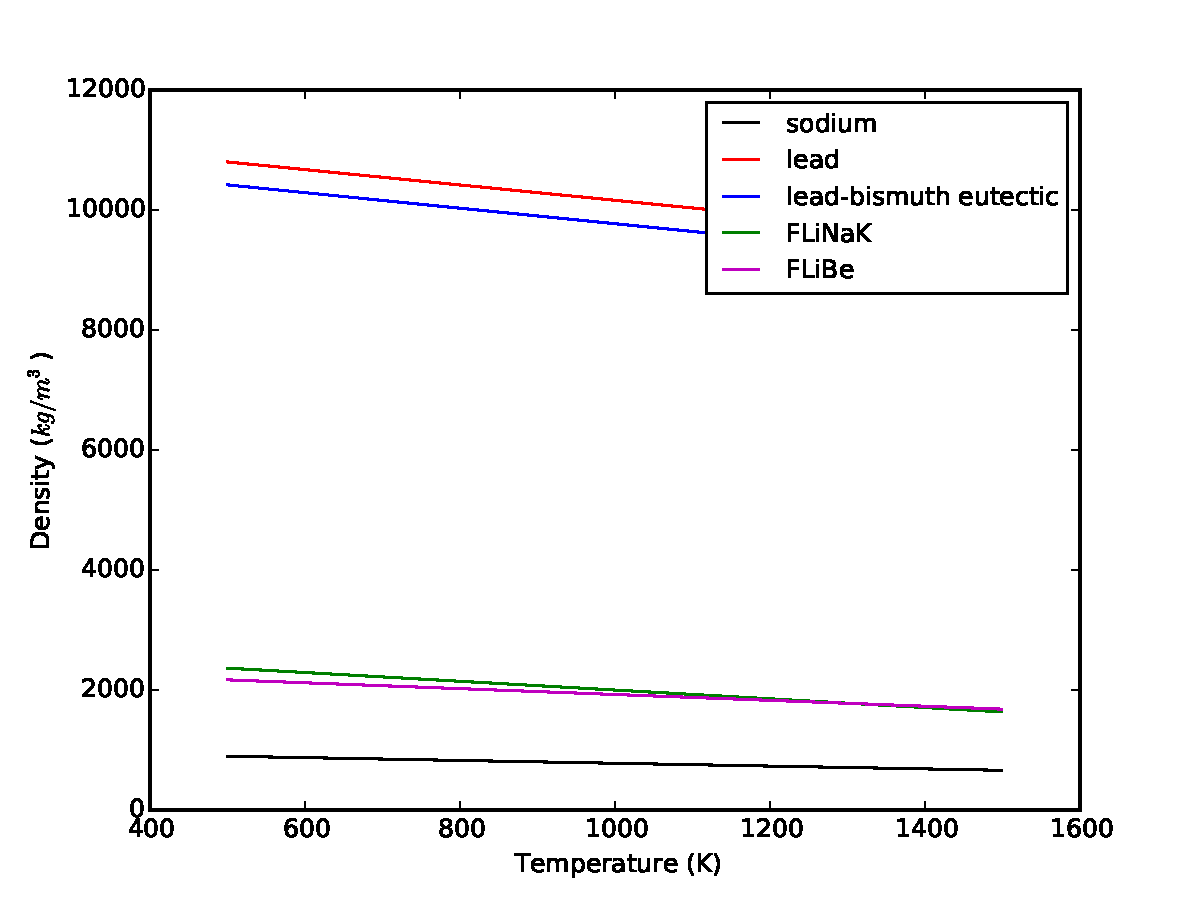
\includegraphics[width=1.0\linewidth]{figures/Densities.pdf}
  \caption{Liquid phases}
\end{subfigure}
\begin{subfigure}{.6\textwidth}
  \centering
  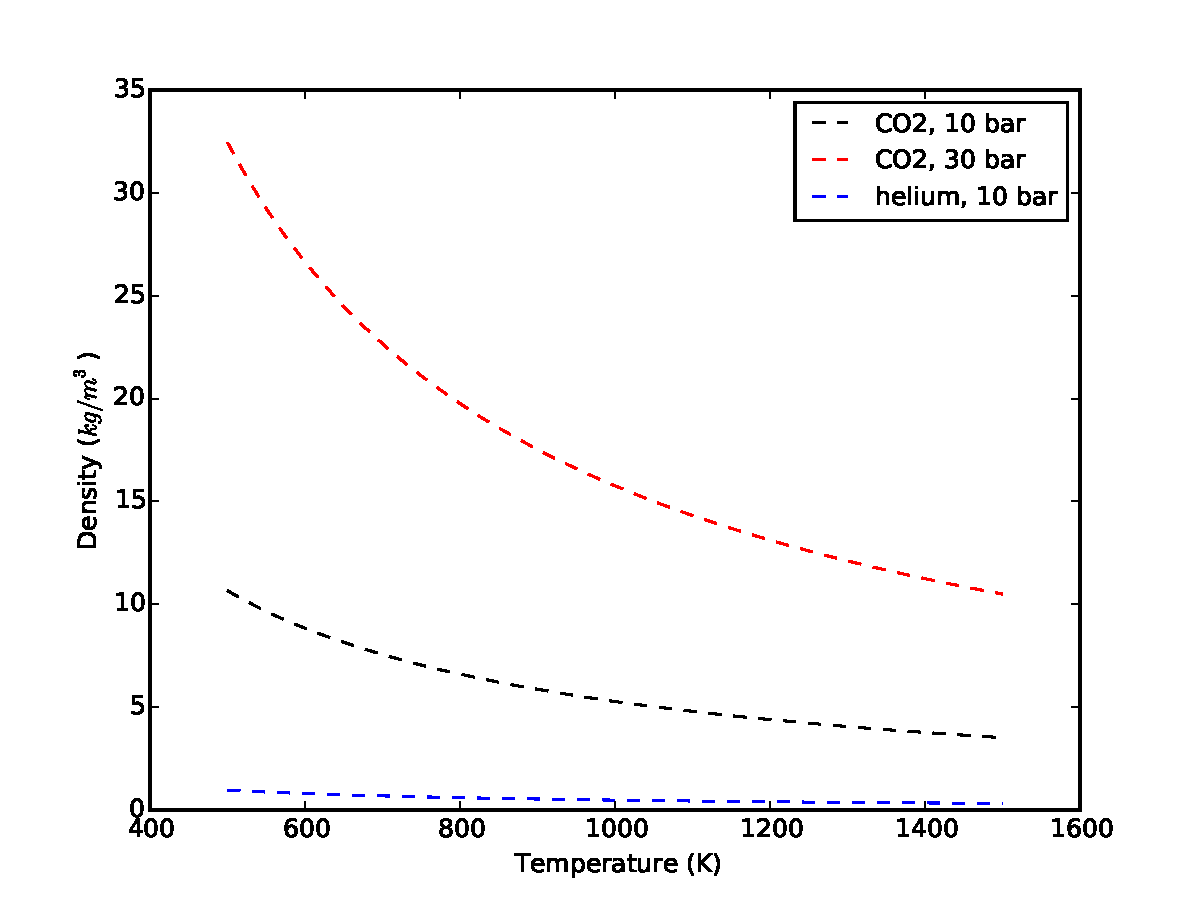
\includegraphics[width=1.0\linewidth]{figures/DensitiesGases.pdf}
  \caption{Gas phases}
\end{subfigure}
\caption{Density as a function of temperature for the (a) liquid and (b) gas phases shown in Table \ref{table:Densities}.}
\label{fig:Densities}
\end{figure}

\subsection{Thermal Conductivity}

The thermal conductivity of all common reactor coolants increases with temperature. Like viscosity, thermal conductivity also increases slightly with pressure, but this effect is nearly negligible. Recommended correlations for thermal conductivity as a function of temperature for the coolants investigated in this section is given in Table \ref{table:ThermalConductivities}. These thermal conductivities as a function of temperature are plotted in Fig. \ref{fig:ThermalConductivities}.

\begin{table}[H]
\caption{Correlations for thermal conductivity (W/m\(\cdot\)K) as a function of temperature (K) for common reactor coolants.}
\centering
\begin{tabular}{l l l c}
\hline\hline
Coolant & Phase & Correlation & Error\\ [0.5ex]
\hline
carbon dioxide						& gas		& tabulated data									& ---\\
FLiBe \cite{saltproperties}				& liquid		& \(k=0.629697+0.0005T\)								& \\
FLiNaK \cite{saltproperties}			& liquid		& \(k=0.36+(5.6\times10^{-4})T\)							& 5\%\\
lead \cite{LMproperties}				& liquid		& \(k=9.2+0.011T\)									& 10\%\\
lead-bismuth eutectic \cite{LMproperties}	& liquid		& \(k=3.284+(1.617\times10^{-2})T-(2.305\times10^{-6})T^2\) 	& 5\%\\
sodium \cite{LMproperties}			& liquid 		& \(k=104+0.047T\) 									& 8\%\\
\hline
\end{tabular}
\label{table:ThermalConductivities}
\end{table}

\begin{figure}[H]
  \centering
  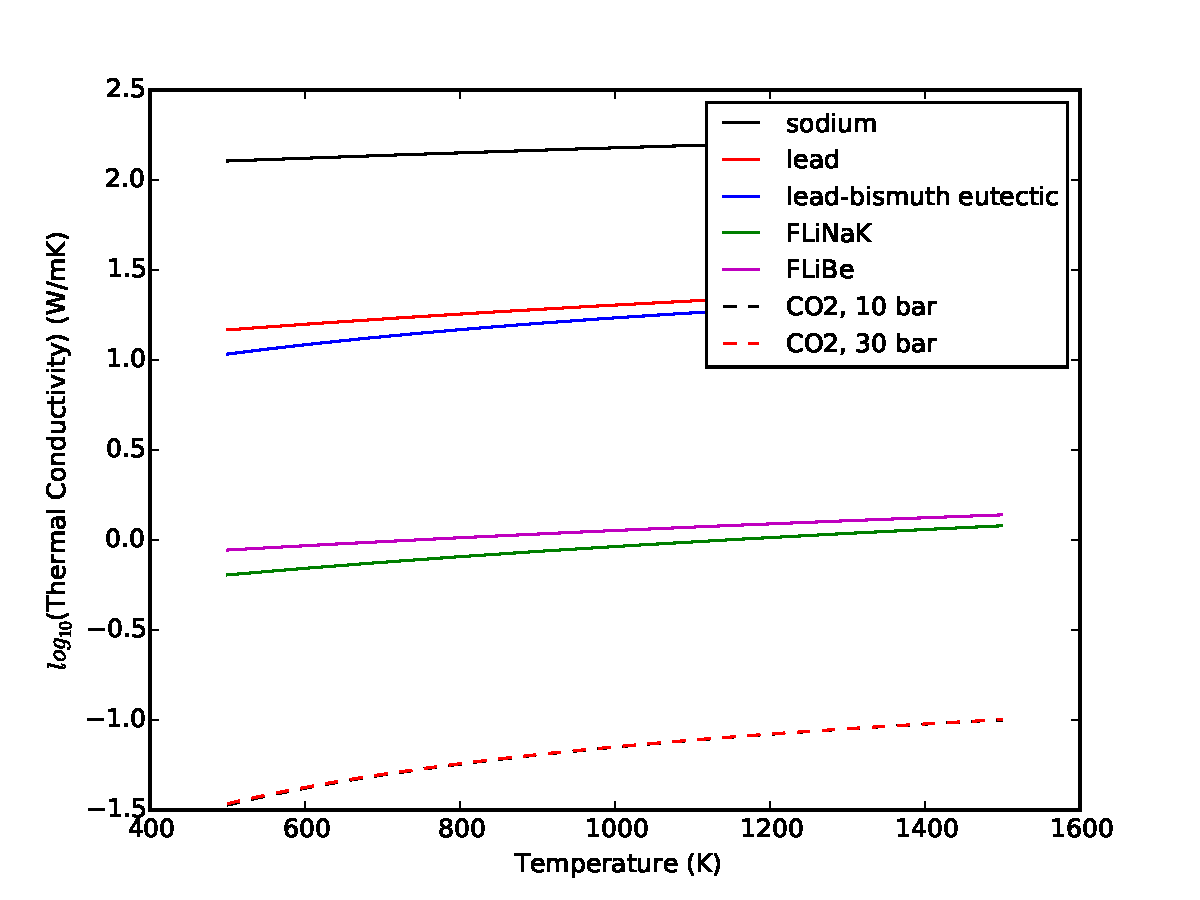
\includegraphics[width=10cm]{figures/ThermalConductivities.pdf}
  \caption{A comparison of thermal conductivity as a function of temperature for the phases shown in Table \ref{table:ThermalConductivities}.}
  \label{fig:ThermalConductivities}
\end{figure}

\subsection{Viscosity}

Fig. \ref{fig:viscosity} shows how dynamic viscosity varies as a function of reduced temperature and pressure for liquids and gases. In the limit of low densities (gases), viscosity increases as a function of temperature. At higher pressures, viscosity decreases as a function of temperature until reaching the critical temperature, beyond which it increases, regardless of pressure. For both liquids and gases, viscosity is relatively independent of pressure, though does increase slightly with pressure. Recommended correlations for viscosity as a function of temperature for the coolants investigated in this section is given in Table \ref{table:Viscosities}. These viscosities as a function of temperature are plotted in Fig. \ref{fig:Viscosities}.

\begin{figure}[H]
  \centering
  \includegraphics[width=8cm]{figures/Viscosity.pdf}
  \caption{Viscosity as a function of reduced temperature and pressure \cite{bird}.}
  \label{fig:viscosity}
\end{figure}

\begin{table}[H]
\caption{Correlations for viscosity (\(Pa\cdot s\)) as a function of temperature (K) for common reactor coolants.}
\centering
\begin{tabular}{l l l c}
\hline\hline
Coolant & Phase & Correlation & Error\\ [0.5ex]
\hline
carbon dioxide							& gas		& tabulated data									& ---\\
FLiBe \cite{saltproperties}					& liquid		& \(\mu=(1.16\times10^{-4})\exp{(3755/T)}\)				& \\
FLiNaK \cite{saltproperties}				& liquid		& \(\mu=(2.487\times10^{-5})\exp{(4478.62/T)}\)					& 2\%\\
lead \cite{LMproperties}					& liquid		& \(\mu=(4.55\times10^{-4})\exp{(1069/T)}\) 				& 4\%\\
lead-bismuth eutectic \cite{LMproperties}		& liquid		& \(\mu=(4.94\times10^{-4})\exp{(754.1/T)}\)				& 5\%\\
sodium \cite{LMproperties}				& liquid 		& \(\mu=\exp{\left(-6.4406-0.3958\ln{(T)}+556.835/T\right)}\) 	& 5\%\\
\hline
\end{tabular}
\label{table:Viscosities}
\end{table}

\begin{figure}[H]
  \centering
  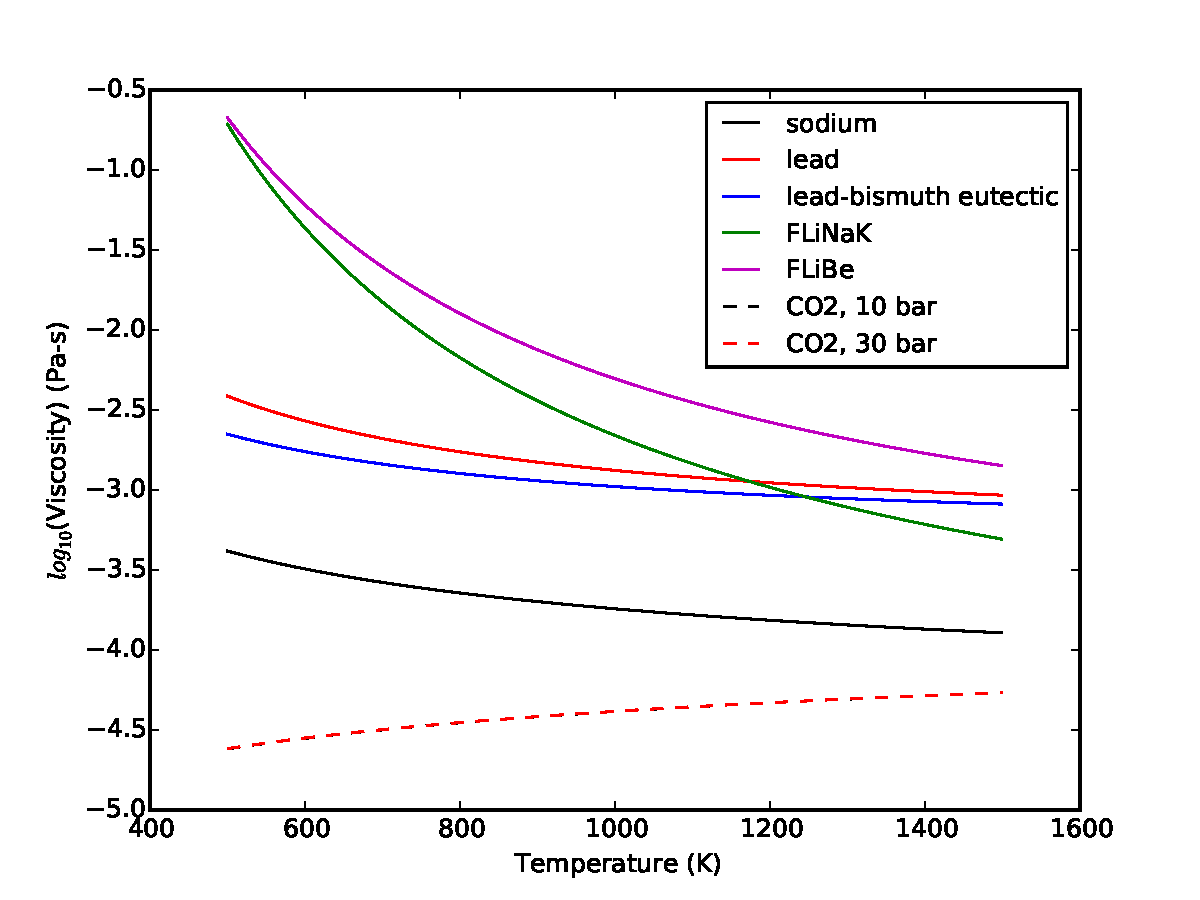
\includegraphics[width=10cm]{figures/Viscosities.pdf}
  \caption{A comparison of viscosity as a function of temperature for the phases shown in Table \ref{table:Viscosities}.}
  \label{fig:Viscosities}
\end{figure}

\subsection{Specific Heat}

Specific heat generally increases with temperature, though the correlations for salt specific heats have high uncertainty. For FLiBe, no simple correlation exists, and many researchers assume a constant value.

\begin{table}[H]
\caption{Correlations for isobaric specific heat (\(J/kg\cdot K\)) as a function of temperature (K) for common reactor coolants.}
\centering
\begin{tabular}{l l l c}
\hline\hline
Coolant & Phase & Correlation & Error\\ [0.5ex]
\hline
carbon dioxide \cite{CO2}				& gas		& tabulated data & ---\\
FLiBe \cite{saltproperties}				& liquid		& \(C_p=2415.78\)														& \\
FLiNaK \cite{saltproperties}			& liquid		& \(C_p=976.78+1.0634T\)												& 10\%\\
lead \cite{LMproperties}				& liquid		& \(C_p=176.2-(4.923\times10^{-2})T+(1.544\times10^{-5})T^2-(1.524\times10^6)T^{-2}\) 	& 7\%\\
lead-bismuth eutectic \cite{LMproperties}	& liquid		& \(C_p=164.8-(3.94\times10^{-2})T+(1.25\times10^{-5})T^2-(4.56\times10^5)T^{-2}\)	& 7\%\\
sodium \cite{LMproperties}			& liquid 		& \(C_p=-(3.001\times10^6)T^{-2}+1658-0.8479T+(4.454\times10^{-4})T^2\) 			& 1\%\\
\hline
\end{tabular}
\label{table:IsobaricSpecificHeats}
\end{table}

\begin{figure}[H]
  \centering
  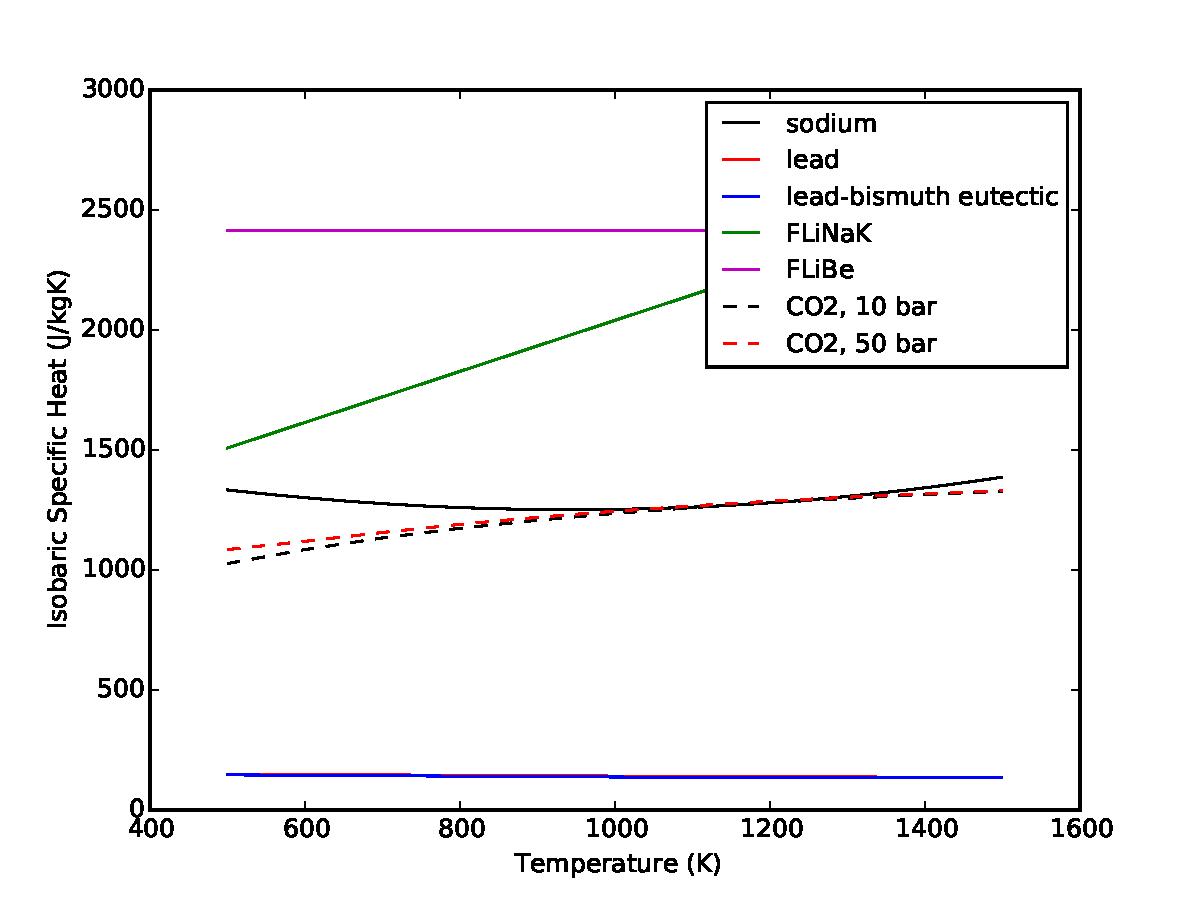
\includegraphics[width=10cm]{figures/IsobaricSpecificHeats.pdf}
  \caption{A comparison of isobaric specific heat as a function of temperature for the phases shown in Table \ref{table:IsobaricSpecificHeats}.}
  \label{fig:IsobaricSpecificHeats}
\end{figure}

\subsection{Surface Tension}

Because the surface tension of gases is even smaller than those for liquids, and because the goal is to motivate neglecting surface tension in the boundary conditions, the data for gas coolants is not needed. If the surface tension of the following liquids can be neglected, then it certainly can be neglected for gases.

\begin{table}[H]
\caption{Correlations for surface tension (N/m) as a function of temperature (K) for common reactor coolants.}
\centering
\begin{tabular}{l l l c}
\hline\hline
Coolant & Phase & Correlation & Error\\ [0.5ex]
\hline
FLiBe \cite{saltproperties}				& liquid		& \(\sigma=0.295778-(0.12\times10^{-3})T\)	& 3\%\\
FLiNaK \cite{saltproperties}			& liquid		& \(\sigma=0.2726-(1.014E-4)T\)			& 2\%\\
lead \cite{LMproperties}				& liquid		& \(\sigma=(525.9-0.113T)\times10^{-3}\) 		& 4\%\\
lead-bismuth eutectic \cite{LMproperties}	& liquid		& \(\sigma=(448.5-0.08T)\times10^{-3}\)		& 3\%\\
sodium \cite{LMproperties}			& liquid 		& \(\sigma=(231-0.0966T)\times10^{-3}\) 		& 6\%\\
\hline
\end{tabular}
\label{table:SurfaceTensions}
\end{table}

\begin{figure}[H]
  \centering
  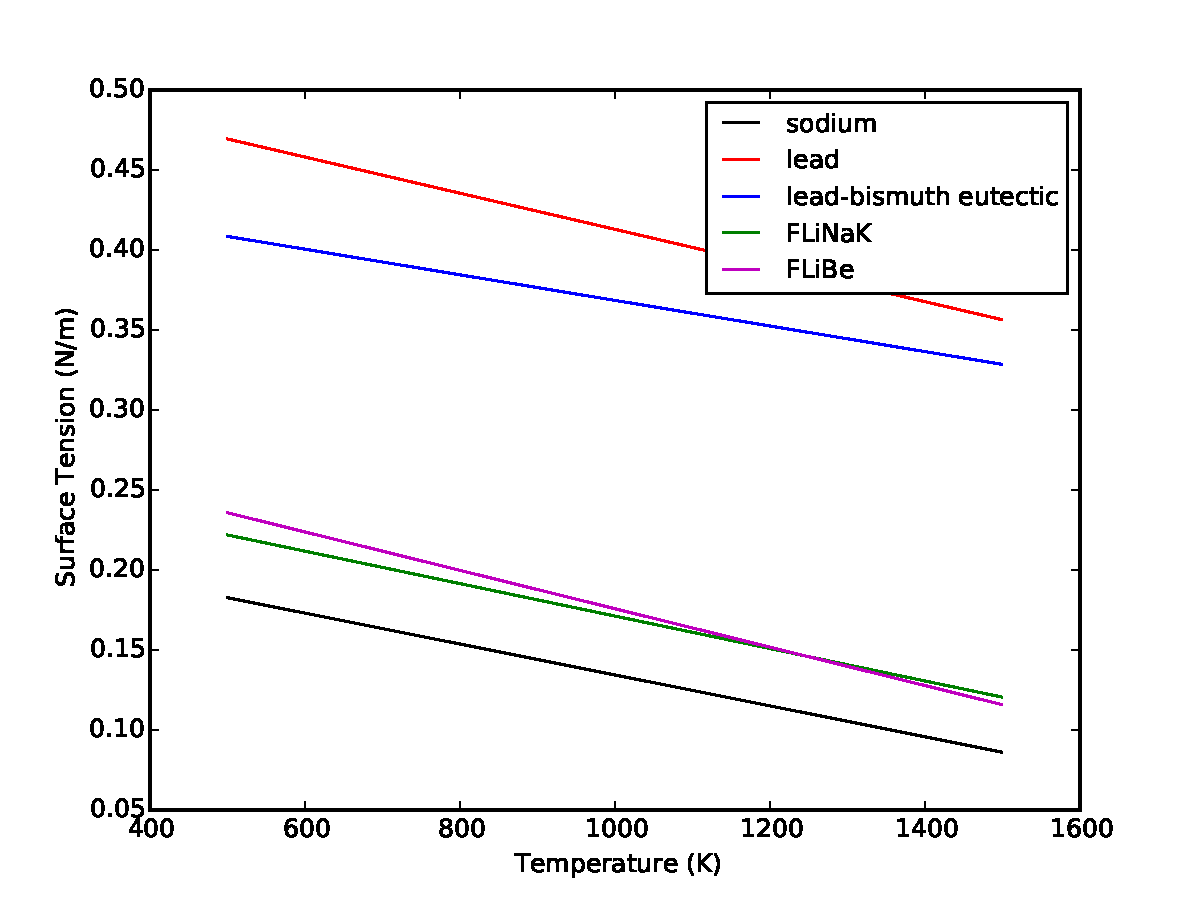
\includegraphics[width=10cm]{figures/SurfaceTensions.pdf}
  \caption{A comparison of surface tension as a function of temperature for the phases shown in Table \ref{table:SurfaceTensions}.}
  \label{fig:SurfaceTensions}
\end{figure}

\subsection{Phase Change}

PRONGHORN does not have the capability to model two-phase flow, and hence should not be used to model transients in which the coolant boils or freezes.

\begin{table}[H]
\caption{Phase change properties for common reactor coolants.}
\centering
\begin{tabular}{l c c l}
\hline\hline
Coolant & Melting Point (K) & Boiling Point (K) & Latent heat of boiling (J/kg)\\ [0.5ex]
\hline
lead \cite{LMproperties}				& 600.6	& 2021	& \(8.586\times10^5\)\\
lead-bismuth eutectic \cite{LMproperties}	& 398.0	& 1927	& \(8.560\times10^5\)\\
sodium \cite{LMproperties}			& 371.0 	& 1155 	& \(4.237\times 10^3\)\\
\hline
\end{tabular}
\end{table}

\section{Carbon Dioxide}

The Atomic Energy Act of 1946 disrupted the international trade of information regarding civilian uses of atomic energy. Other countries could not access the enrichment knowledge held by the United States. In order to build thermal reactors, the constraint that the fuel had to be natural uranium severely restricted the coolant-moderator choices available to the French and British. Heavy water was too expensive, and helium reserves or atmospheric distillation technology were not available, and hence these countries developed carbon dioxide-cooled gas reactors using metallic, natural uranium fuel.

These reactors operated at relatively low temperature due to interactions of carbon dioxide with graphite at high temperature. At around 600 \degree C, carbon dioxide dissociates into carbon monoxide and oxygen gas. The oxygen oxidizes graphite and metallic structures, a process that can be mitigated by introducing methane, since methane dissociates into carbon and hydrogen gas (where the hydrogen gas combines with the oxygen to produce water vapor). Another negative aspect of the design is the relatively poor heat transfer characteristics of carbon dioxide, which necessitated using fins on the metal cladding. This, combined with the problems associated with carbon dioxide dissociation, motivated the use of helium in future gas reactors. Table \ref{table:CO2Reactors} gives typical operating conditions for several carbon dioxide reactors. In total, there were 37 MAGNOX-class reactors and 15 Advanced Gas Reactors (AGRs) operated in Europe. 

\begin{table}[H]
\caption{Operating conditions for several carbon-dioxide-cooled reactors \cite{MAGNOX}. All material properties are evaluated at the median of the operating temperature range.} % ADD IN AGRs
\centering
\begin{tabular}{l l l l}
\hline\hline
 & Calder Hall & Hinkley Point & Wylfa\\ [0.5ex]
\hline
 Power (MWth)						& 182				& 980				& 1875\\
 Core D (m)						& 9.45				& 14.9				& 17.4\\
 Pressure (MPa)					& 0.7					& 1.22				& 2.62\\
 Temperature (C)					& 140/336				& 180/375				& 247/414\\
 Flowrate (kg/s)						& 891				& 4536				& 10254\\
 Velocity (m/s)						& 20.0				& 					& \\
 \(\rho\) (kg/\(\textrm{m}^3\))			& 7.58				& 12.12				& 23.64\\
 \(\mu\) (\(10^{-5}\) Pa\(\cdot\)s)			& 2.43				& 2.60				& 2.81\\
 \(k\) (W/m\(\cdot\)K)					& 0.034				& 0.038				& 0.042\\
 \(C_p\) (J/kg\(\cdot\)K)				& 1017.5				& 1104.0				& 1078.5\\
 \(\beta\) (1/K)						& & &\\
 \(D\) (m)							& \(2.48\times10^{-2}\)	&					& \\
 \(Pr\)							& 0.71				& 0.72				& 0.72\\
 \(Br\)							& \(1.5\times10^{-3}\)	& & \\
 \(Ec\)							& \(2.0\times10^{-3}\)	& & \\
 \(Re\)							& \(1.6\times10^5\)		& 					& \\
 \(Pe\)							& \(1.2\times10^5\)		& 					&\\
 \(Br/Pe\)							& \(1.2\times10^{-8}\)	& & \\
 \(\beta Ec\)						& & & \\
 \(We\)							& & & \\
\hline
\end{tabular}
\label{table:CO2Reactors}
\end{table}

\section{General Considerations}

Sodium is the best coolant for reactors.

Liquid metals: 

\begin{itemize}
\item Relatively costly, but due to their excellent heat transfer characteristics, a relatively small volume is needed, somewhat negating this claim
\item High thermal conductivities introduce the possibility of thermal shock in transients
\item High induced radioactivities, meaning that an additional heat transfer loop is often included to shield the power conversion side of the plant from radiation, reducing the overall thermal efficiency. However, due to the small coolant volume in the core region and the higher flowrates encountered in liquid metal reactors than in thermal reactors, the induced radioactivity is usually lower than in thermal reactors. 
\item High chemical reactivity, requiring special materials for surfaces that contact the fluid
\end{itemize}

\begin{itemize}
\item Resistant to radiation damage, so they have low replenishment costs
\item High boiling point and low vapor pressure means high outlet temperatures can be achieved with near atmospheric pressure
\item High thermal conductivities reduce hot spots and reduces structural warping
\end{itemize}

\section{Helium}

Because higher temperatures permit higher efficiencies, while also extending applicability to process heat generation, helium was adopted for gas-cooled reactors to avoid the problems associated with the dissociation of carbon dioxide at high temperature. Helium has been proposed for use in both thermal and fast reactors. High Temperature Gas Reactors (HTGRs) are defined to be thermal reactors using ceramic fuel, a graphite moderator, and helium. Hence, while the carbon dioxide reactors did use gas and operated at relatively high temperature, they are not considered to be HTGRs. All thermal reactors that have used or are proposed to use helium fall under the HTGR category. 

Fast reactors using helium are referred to as Gas-Cooled Fast Reactors (GCFRs).

The terminology used for gas-cooled reactors is necessarily different because many components are specifically designed for gases, rather than liquids. 

\subsection{High Temperature Gas Reactors (HTGRs)}

Seven HTGRs reactors have operated in the world - five of these were experimental or prototype reactors, while two were commercial-scale demonstrations \cite{HTGRLessonsLearned, PNNLReport}. All of these reactors use ceramic fuel (coated particle), graphite moderator, and water as the secondary coolant. Ceramic materials and an inert coolant are required to avoid chemical-interaction temperature limitations that would prevent high-temperature operation, such as is the case for carbon dioxide dissociation at high temperature.

Four of these reactors use prismatic fuel, while three use pebble fuel. There is no significant advantage of one fuel type over the other \cite{PNNLReport}.

Fig. \ref{fig:HTGRTimeline} shows an operating timeline of these seven HTGRs.

\begin{figure}[H]
\centering
\includegraphics[width=0.6\linewidth]{figures/HTGRRecord.pdf}
\caption{Timeline of HTGR operation (source: http://www.jaea.go.jp/jaeri/english/ff/ff43/randd01.html).}
\label{fig:HTGRTimeline}
\end{figure}

In addition to these plants, several conceptual designs have been developed in the United States. Between 1971 and 1974, General Atomics sold five HTGR plants, but these were never built. 



 
Helium is non-corrosive and has higher thermal conductivity than carbon dioxide. In addition, due to the lower flowrates of helium required, there are lower flow-induced vibrations.

The cost of helium purification and storage is a negative aspect of the design, but relatively high power densities can be attained, which allows smaller reactor vessels and structural inventories. The absence of metallic cladding is a benefit in these thermal systems due to their lower parasitic absorption cross sections.

Friction and wear between components in the high-temperature helium environment can be mitigated by applying molybdenum disulfide lubricant.

Virtually all initial fuel cycles focused on the highly-enriched U-235/Th fuel cycle. In this cycle, sometimes referred to as the Feed-Breed system, two different fuels are present in the core. The breed fuel, comprising about 75\% of the core, contains a mixture of U-235 and Th-232, and the consumption of U-235 is nearly balanced by the production of U-233. This fuel is reprocessed at frequent intervals. The feed fuel in the remainder of the core contains highly-enriched U-235. The feed fuel was refueled on-line through vertical motion developed for the AGR, while the breed fuel was reprocessed on the typical two to three year schedule. 

An alternative fuel cycle using low-enriched uranium provides fuel cycle costs comparative to the Feed-Breed design. By designing a core with appropriate heterogeneity, sufficient self-shielding of U-238 resonances could be obtained.

Although reprocessing of coated particle fuels is difficult, the U-235/Th fuel cycle can still produce relatively low fuel cycle costs.

Many of the reactor designs employ downwards flow of helium through the core, which is opposite the case for the majority of other reactor designs. This design choice was originally made to allow online refueling of prismatic block elements in Dragon. Downwards flow prohibits natural circulation cooling, but the low density of helium makes this insignificant, since the temperatures in a transient are more strongly controlled by the thermal inertia of the graphite. 

\subsubsection{Dragon}
The United Kingdom Dragon test reactor was the first HTGR built in the world, and was intended for testing of fuel and materials \cite{Dragon}. This was the first reactor to use cold coolant to maintain the vessel at sufficiently low temperatures such that creep did not cause significant deformation. This design has been incorporated into the more advanced gas reactor designs. In addition, for components that touch the hot gas, metal insulation prevented excessive temperatures. 

Dragon initially operated on highly-enriched fuel (about 93\% enrichment), but due to concerns over availability, switched to low-enriched (about 3.5\%) fuel. Many later HTGR designs would continue to use highly enriched fuel, but the ability to use low-enriched fuel is encouraging due to the long lead time expected for commercial availability of higher-enriched fuels.

The initial expectation of coated particle fuel was that it would exhibit high release rates of fission product gases in order to remove fission product poisons and improve the neutron economy. Hence this reactor was designed with a coolant purification system to remove fission products. The actual release rates were too low to provide any neutronics benefit, and hence a different approach in the fuel design was pursued. From then on, coated particle fuel was to be developed. While a leak-tight primary system is not required for dose reasons, it is required to prevent excessive helium loss.

The reactor contained hexagonal fuel elements surrounded by a graphite reflector that was machined on one side to be flush with the fuel assemblies, and on the periphery to form a circular boundary. Control rods entered in the reflector. The fuel was 2.54 m tall, but only the center 1.6 m contained fuel - the ends were reflectors.

Due to the strong negative temperature coefficient, power could be controlled by manipulating the helium flowrate. 

Due to the low thermal inertia of the core, the steam generators had to be located at a higher elevation than the reactor to permit natural circulation cooling. A leak in a steam generator could introduce significant quantities of water into the reactor core, where it might be possible that the upward flow of helium could hold the water in the core for a sufficient length of time to cause a power excursion. The possibility of positive reactivity insertion is greater for small test reactor with relatively high neutron leakage, since one of the positive contributions due to water is a reduction in leakage. Hence, to ensure that no power excursion were possible, a lithium sulphate poison was added to the secondary coolant. Despite low corrosion rates in experimental tests, in practice, high corrosion rates were observed, and the inclusion of a protective poison led to more steam generator leaks than had the solute not been included. In all of these cases, helium leaked into the secondary loop due to the pressure differential. 

\subsubsection{Peach Bottom Unit 1}
The Peach Bottom Unit 1 reactor was designed by General Atomics and was the first HTGR in the United States \cite{PeachBottomFuel}. Peach Bottom utilized two different fuel types during operation. The first core loading used a very simple coated fuel design - the kernel was coated in a single layer of pyrolitic carbon. About 90 fuel elements failed with this fuel, prompting the development of BISO fuel, which features an additional buffer layer to protect the pyrolitic carbon layer. In the simpler coated-particle fuel designs, the kernel experienced an ``amoeba effect,'' whereby it would propagate through the particle and eat through the containing layers due to strong temperature gradients. To further enhance fission product retention, future HTGRs used TRISO fuel, which added the SiC layer. Rhodium was included in the fuel in order to obtain a prompt negative fuel temperature reactivity coefficient.

The fuel was a solid, cylindrical element with a total height of 3 m and 8.9 cm in diameter. 2.26 m of this height was annular fuel compacts, with the surrounding portions containing an upper and lower reflector and an internal fission product trap below the lower reflector. Spacer rings located at the top of the assembly maintained the pin pitch. These fuel rods were spaced individually throughout the core - there were no assemblies of fuel rods, nor hexagonal prismatic blocks.

The helium flowed upwards through the core, a characteristic uncommon to helium-cooled reactors. Because upflow corresponds to the same direction as buoyancy forces, Peach Bottom could utilize natural circulation cooling for decay heat removal. Another unconventional aspect of the design was that the control rods inserted from the bottom, which required substantial reliability evidence for licensing. Bottom-insertion control rods require less materials considerations due to the lower temperatures in the bottom of the core than the top. Pipes contained metallic thermal barriers to prevent direct contact between the hot helium and the metals.

\subsubsection{AVR}
The AVR reactor in Germany was the first reactor to use spherical fuel, and was primarily used to test different fuel designs and demonstrate the principles of high temperature reactor operation \cite{AVRTheenhaus}. The AVR successfully operated at 1000\degree C, the highest temperatures in a commercial reactor to date. Like in all subsequent pebble bed designs, the fuel pebbles circulate through the reactor multiple times before final discharge. Gamma spectrometers are used to evaluate the burnup of pebbles, and reintroduce the pebbles provided their burnup is lower than the acceptable limit. 

About 10 years into the operation, a leak developed in one of the steam generators. Because the steam generators were located at an elevation above the core (also within the pressure vessel), this led to several tons of water being introduced into the core. Because the reactor did not have a low-point drain to easily remove the water, the water was removed over a 15-month period, but without removing the fuel. This moisture ingress accident became one of the design-basis accidents of the THTR. Current HTGR designs locate the steam generator lower than the core in order to reduce siphoning effects that would further introduce water into the core from a steam generator tube leak. In addition, the steam generator and helium compressors tend to be located outside of the pressure vessel altogether.

Instrumented graphite spheres containing metal wires with known melting points, were used to conclude that in a depressurized LOFC transient, the pebble fuel would remain below failure temperatures even without control rod insertion.


The very high retention of fission products in the fuel was not anticipated, and hence the design of this reactor over-compensated by having two pressure vessels. No damage was observed in the graphite reflectors, but due to the dark color of graphite, visual inspection was very difficult. One of the most complicated issues was graphite dust propagation.

During initial loading, the pebble packing fraction was higher than expected, and more than expected fuel failures occurred. To lower the packing rate, the damaged fuel was removed as the fuel cycled through the core.

Generally, uranium consumption in HTRs using TRISO fuel is similar to consumption in LWRs using reprocessing. AVR discharged 50-100 fuel pebbles per day. These pebbles were packaged in stainless steel canisters and held in a spent fuel pool. After a cooling time of about two years, they are transferred to dry cask storage. Unfortunately, reprocessing of TRISO fuel is not economical.

\subsubsection{Fort St. Vrain (FSV)}
The FSV reactor was designed by General Atomics, and is similar in layout to the GT-MHR design. This reactor experiences major complications, primarily due to core instabilities and ingress accidents. For the first several years of operation, power levels above 70\% rated power led to core instabilities, most likely due to small movements of the fuel and reflector components which were caused by temperature gradients and bypass flow. By installing restraining devices in the core, these power fluctuations were largely eliminated. The core contained 37 individually-regulated flow regions with orifices to equalize the core outlet temperature distribution. 

FSV experienced many water ingress accidents, either from the steam generator or from water lubricant of circulator bearings, and demonstrated the many ways in which water ingress can negatively impact plant performance. This water either induced immediate consequences, or would leach into cracks and release over long periods of time to induce long-term consequences. A reactor drain would have helped remove this water ingress. The associated complications at Fort St. Vrain due to water ingress included:

\begin{enumerate}
\item Corrosion of carbon steel components, which in one transient prevented six control rods from entering
\item Degradation of the reserve shutdown control system - several hoppers full of borated balls failed to open
\item Water-induced leaching of boron between adjacent borated balls over long periods of time caused the balls to crystallize together, making reliable operation uncertain
\item Addition of positive reactivity. The net reactivity effect of water may be either positive or negative, depending on the amount of water present. Smaller amounts of water tend to add positive reactivity. Because water parasitically absorbs more neutrons than graphite, there is some negative component. Positive contributions include:
	\begin{enumerate}
		\item Increased resonance escape probability, since neutrons lose more energy per collision with hydrogen than carbon
		\item Cooling of the graphite and fuel, introducing reactivity due to the Doppler effect
		\item Higher nonleakage probability due to the increased overall fluid density
	\end{enumerate}
\item Natural presence of water in graphite, requiring large amounts of time at high temperature for water to outgas from the graphite even if no ingress accident occurred
\end{enumerate}

FSV was finally shut down when its owner decided that the cost to replace cracking steam generators was too high. The FSV reactor did not even reach break-even due to the many complications experienced during operation. A cost analysis is complicated by the fact that the fuel assembles used only had one manufacturer, General Atomics, which distorted the price to a potentially high-than-free-market price.

\subsubsection{THTR}
During operation, many fuel pebbles were damaged due to control rod insertion directly into the bed in unfavorable conditions.

THTR was shut down after only about one year of power operation due to a number of reasons, including environmental group actions, the fuel manufacturer ceasing to produce fuel pebbles, and economic uncertainty.

\subsubsection{High Temperature Test Reactor (HTTR)}
HTTR is located on the Japanese Atomic Energy Agency research campus. 

Unexpected changes in bypass flows produced hot spots.

\subsubsection{HTR-10}\cite{HTGRLessonsLearned}


The movement of pebbles along the graphite and rubbing together of the graphite reflector blocks causes the graphite to wear and produce graphite dust. These particles either collect in the bottom of the core or heat transfer surfaces such as in the steam generator, reducing efficiency. In addition, fission products that escape the fuel tend to bind onto the graphite dust, and hence may become mobile in depressurization accidents.

Due to the requirements to have a high-purity helium environment, but with a high reliability for control rod insertion, there is a limitation on what materials can be used as lubricants for the control rods. Conventional oil lubricant could not be used due to the high temperature environment. Molybdenum disulfide was selected as the lubricant.
 
\subsubsection{MHTGR}\cite{HTGRLessonsLearned}
This conceptual design placed eight reactors on each site, with the generation of electricity primarily considered as a byproduct.

\subsubsection{GT-MHR}\cite{HTGRLessonsLearned}
The GT-MHR is a commercial design developed by General Atomics that uses a gas turbine to generate power instead of a steam generator. This design features a connection from the reactor pressure vessel to the power conversion vessel, and the definition used for this connection has varied from design to design, with some vendors referring to the connection as a ``vessel,'' and others as a ``pipe.'' The distinction impacts the level of regulatory oversight needed for that component. Peach Bottom, HTTR, and HTR-10 have not defined this component in a consistent manner.


The experience gained from these deployments of HTGR designs has led from the transition of the use of prestressed concrete reactor pressure vessels to metal vessels due to complications associated with bacterial corrosion of structural tendons in the concrete. In addition, while earlier designs tended to have cores with approximately equal height and diameter for neutron leakage concerns, later designs incorporated substantially taller cores to facilitate natural circulation for fully passive heat removal. In order to keep fuel temperatures below their failure temperatures, more modern designs, for both pebble and prismatic fuel, use an annular core structure, though are still limited to about 600 MWth. Conceptual designs that have evolved out of past HTGR experience include the PBMR, GT-MHR, MHTGR, Antares, and EM-2 designs.
 

The viscosity of gases increases with temperature. In accident conditions, hot channels produce even greater friction coefficients, further reducing flow in a positive feedback loop.

Tritium is produced from interactions of He-3 with neutron irradiation (though this effect is small if the core volume of helium is kept small) and from B-10 and Li-6 impurities in the graphite.

Helium generally flows downwards in HTGRs, which essentially prevents any effective natural circulation cooling. In addition, in transients, the fuel must be cooled very quickly to avoid flow instabilities and graphite corrosion in the case of water ingress accidents, which limits the extent to which the core can rely on passive safety, since it would take too long for the fuel to cool by the negative temperature coefficient.

\subsubsection{Summary}

In summary, complications that have arisen from the operation of HTGRs include:

\begin{enumerate}
\item Oil and water ingress into the core, arising primarily from lubrications on helium compressors and circulators.
\end{enumerate}

To date, all HTGR reactors have been financially unsuccessful, including the two commercial-scale plants Fort St. Vrain and THTR. Reliability was good for the smaller plants, but for larger plants such as Fort St. Vrain, capacity factors were low.

However, from a technical point of view, the radiological source terms were lower than LWRs, and the high thermal inertia of graphite and larger margins to fuel failure may indicate improved inherent safety as well. 

Complications associated with high-temperature reactors in general include:

\begin{enumerate}
\item Continued exposure to temperatures above 1000 \degree C may lead materials to have useful lives of only five to ten years \cite{PNNLReport}.
\end{enumerate}

\clearpage
\begin{sidewaystable}
\begin{table}[H]
\caption{Operating conditions for several helium-cooled reactors \cite{HTGRLessonsLearned}. All material properties are evaluated at the median of the operating temperature range. Note that the parameters shown in the third and fourth sections are very approximate, and only reflect expected values over normal operating conditions.}
\centering
\begin{tabular}{l l l l l l l l l l}
\hline\hline
 								& Dragon 		& Peach Bottom & AVR 		& FSV		& THTR 		& HTTR 		& HTR-10 	& MHTGR 	& MH-GTR\\ [0.5ex]
\hline
 Power (MWth)						& 21.5		& 115		& 46			& 842 		& 750		& 30			& 10			& 350		& 600\\
 Density (MW/\(m^3\))				& 14.0		& 8.3			& 2.6			& 6.3			& 6.0			& 2.5			& 2.0			& 5.9			& 6.5\\
 \hdashline
 Fuel	 							& prismatic	& prismatic	& pebble		& prismatic	& pebble		& prismatic	& pebble		& prismatic	& prismatic\\
 								& 			& Th/U(235)-C\\
 Enrichment (wt\%)					& 3.5			& 93			& 93			& 93			& 93			& 3-10		& 17			& 19			& 19\\
 \hdashline
 \(P\) (MPa)						& 2.0			& 2.3			& 1.1			& 4.08		& 4.0			& 4.0			& 3.0			& 6.4			& 7.0\\
 Secondary \(P\) (MPa)				& 1.58		&			&			&			&			&			&\\
 Temperature (C)					& 350/750		& 327/726		& 250/950		& 404/777		& 250/750		& 395/950		& 250/700		& 258/686		& 491/850\\
 Flowrate (kg/s)						& 9.6			& 60.0		& 12.7		& 110.0		& 298		& 10.2		& 3.2			& 158.0		& 320.0\\
 Flow direction						& up			& up			& up\\
 \hdashline
 Velocity (m/s)						& 			& 60			& 			& 			& 12\\
  \(D\) (mm)						&			& 11.6		&			& 			& 26\\
 \(\rho\) (kg/\(\textrm{m}^3\))			&			& 1.38		& 			&			& 2.47\\
 \(\mu\) (\(10^{-5}\) Pa\(\cdot\)s)			& 			& 3.94		& 			&			& 3.85\\
 \(k\) (W/m\(\cdot\)K)					& 			& 0.31		& 			&			& 0.30\\
 \(C_p\) (J/kg\(\cdot\)K)				& 			& 5194		& 			&			& 5195\\
 \hdashline
 \(Pr\)							& 			& 0.66		& 			&			& 0.67\\
 \(Br\)							&			& \(1.1\times10^{-3}\)		& & 			& \(3.7\times10^{-5}\)\\
 \(Re\)							&			& \(2.4\times10^{4}\)		& &				& \(2.0\times10^4\) \\
 \(Pe\)							&			& \(1.6\times10^{4}\)					& &	& \(1.3\times10^4\)\\
 \(Br/Pe\)							& 			& \(6.8\times10^{-8}\)	&	&			& \(2.8\times10^{-9}\)\\
\hline
\end{tabular}
\label{table:HeliumReactors}
\end{table}
\end{sidewaystable}

\section{Lead}

Though sodium is the current primary choice for fast reactor systems, lead, and certain alloys of lead including lead-bismuth eutectic (LBE), are generally considered to be the coolants of future fast reactor systems. Lead has a lower melting temperature than sodium, which results in lower corrosion rates and easier maintenance. Sodium is much closer to the commercialization stage than lead, however. The use of LBE is also complicated by the polonium activation products produced by neutron capture in bismuth.

\section{Salts}

Salts have even higher heat capacities than helium, and because both helium- and salt-cooled reactors tend to contain high quantities of graphite, salt \gls{htgr}s tend to have higher effective heat capacities that even further prolong transients. Longer simulation times further necessitate fully implicit solvers and stabilization. 

Due to the higher volumetric heat capacity of salts, their use as reactor coolants is primarily motivated by a greater possible heat removal rate, allowing higher power densities for a given coolant volume. Salt reactors also tend to have relatively high recirculation flows in accident scenarios, and the bypass fraction of total core flow becomes a less important feature in assessing the core temperature than in gas-cooled reactors \cite{AHTR}. 

The viscosity of liquids decreases with temperature, producing a self-regulating temperature effect in accident conditions that is not obtained with gas coolants. 

\section{Sodium}

Sodium is the primary coolant choice for fast reactor systems due to its high volumetric heat capacity, which permits a high power density with a low coolant volume fraction. Sodium is also the cheapest of the potential liquid metal coolants, and can be bought in solid brick form. Sodium has excellent corrosion properties, but reacts chemically with air and water, which requires a tightly-sealed system. In addition, a melting point above room temperature requires guard heating of all piping to prevent freezing. Sodium is compatible with a wide range of materials. 

All naturally-occurring sodium is comprised of Na-23. Sodium becomes activated by neutron irradiation, producing Na-24. Na-24 emits strong gamma rays with a 15-hour half life. 

There are two major types of fast reactors - pool type and loop type. In pool type reactors, the entire primary circuit is submerged in sodium. The intermediate heat exchangers, which exchange heat from the primary loop to the secondary loop, as well as the primary coolant pumps, are submerged in sodium within the reactor pressure vessel. The roof of the vessel is an extremely complicated component due to the fact that it holds the weight of the entire primary circuit - the reactor vessel only holds the weight of the sodium. Pool type reactors generally enjoy better passive safety features, since the very large volume of coolant provides high thermal inertia - in unprotected transients, it is estimated that there would be a ten minute period before the coolant would begin to boil. However, insulating the roof from the hot sodium is a complicated task. The cover gas provides some of this insulating effect. Sodium evaporates at the cover gas-sodium interface. Because the reactor vessel roof is cooler than the sodium, the sodium then condenses on the roof, producing sodium ``fog'' within the cover gas. This fog actually reduces the radiation heat transfer, further shielding the roof. 

The other reactor type, the loop type, has a configuration similar to a conventional plant, where the coolant leaves the reactor vessel to exchange heat to the secondary loop. Pumps are also housed outside the reactor vessel.

Due to the low vapor pressure of sodium, all sodium reactors operate very near atmospheric pressure. A slight pressurization exists to ensure that any leak goes out from the primary coolant. 

All reactors using sodium are fast reactors. Fig. \ref{fig:FastReactorTimeline} shows a timeline of all fast reactors (not just those using sodium); this figure is placed in this section because the majority of these reactors used sodium. 

A substantial difference between fast reactors and thermal reactors is that, while thermal reactors are design in a most-reactive configuration (any change in geometry introduces negative reactivity, fast spectrum reactors can experience increases in reactivity due to core geometry changes. 

Fast reactors tend to contain in-vessel core debris catchers to contain post-accident debris. 

The cores tend to be designed using radial zones (usually two) surrounded by axial and radial blankets. 

Another significant distinction amongst fast reactors is the fuel choice. While many reactors use oxide fuels, several use metal fuels. Metal fuel introduces relatively large thermal expansion, allowing negative reactivity feedback. 

\begin{figure}[H]
\centering
\includegraphics[width=0.6\linewidth]{figures/FastReactorRecord.pdf}
\caption{Summary of all fast reactors designed or built. Only two of these reactors do not use sodium - Clementine uses mercury, and the DFR uses NaK.}
\label{fig:FastReactorTimeline}
\end{figure}

\subsection{Sodium-Cooled Fast Reactors}

While other coolants have been proposed for fast reactors besides sodium, sodium is nearly universally proposed for liquid-cooled fast reactors, and hence the discussion of the thermal physics aspects of fast reactors is held in this section. Fast reactors have much higher neutron flux levels and power densities than thermal reactors. 

\subsubsection{Fuel}
The fuel consists of stacks of fuel pellets housing in metal cladding, a design very similar to traditional \gls{lwr} fuel. Springs internal to the fuel, usually at the top of each rod, hold the pellets in place during shipment. The outer diameters of the cladding in fast reactors are typically in the range of 6 - 8 mm. Each fuel pellet is about 6 mm in diameter with a nearly equal height. 

Several different fuels have been used in fast reactors, though the most common fuel is UO\textsubscript{2}-PuO\textsubscript{2} is the most common. UC-PuC is a second ceramic that has also been used, and a third ceramic in the form of Th-U\textsuperscript{233} has been proposed. Fast reactor designs originating in the United States tend to use metallic fuel, and the use of metallic fuel is becoming more prevalent in modern fast reactor designs. 

The fuel pin design is substantially different from the design of an LWR pin. Due to the fast neutron spectrum, substantially more fission gases are released, and hence a much greater portion of a fast reactor fuel rod must be devoted to a gas plenum. In an LWR, about 90\% of the fuel rod contains fuel, while in a fast reactor, only about one third of the rod contains fuel. Fast reactor cores are generally very squat in order to increase leakage, so the total heigh of the fuel assemblies is approximately the same between LWRs and fast reactors. The gas plenum length is approximately equal to the height of the active core region, and this plenum can be located either above or below the core. The location of the gas plenum in \gls{lwr}s is consistently located above the core, but this location varies in fast reactor designs. Some reactor designs even have plenums both above and below the fuel. If the plenum is above the fuel, then gas leakage immediately leaves the core region, reducing the risk of a reactivity transient. However, at the top of the core, the gas is at the highest temperature, and requires a larger volume (think ideal gas law) for storage than would be required in the cooler region below the core. However, it is not universally the case that a plenum below the core would provide for a smaller total assembly height. Because control rods typically enter from the top of the core, the control ducts extend far above the core to accommodate the withdrawn control rods. It may be preferable for this region above the core to house a larger gas plenum. 

The pellets that comprise the active core region and blanketed on top and bottom by axial blankets, comprised of depleted uranium oxide. The top and bottom blanket are each about 0.3 - 0.4 m high. A schematic of two fuel rod designs is shown in Fig. \ref{fig:FastReactorPins} for a fission gas plenum (a) above and (b) below the fuel pellets. 

\begin{figure}[H]
\centering
\includegraphics[width=0.6\linewidth]{figures/FastReactorPins.pdf}
\caption{Representative fast reactor fuel pin designs for (a) CRBRP and (b) Super Ph\'{e}nix \cite{FastReactors}.}
\label{fig:FastReactorPins}
\end{figure}

Fig. \ref{fig:FastReactorPlenumChoices} shows how the design choice of plenum location has varied over several representative fast reactors.

\begin{figure}[H]
\centering
\includegraphics[width=0.6\linewidth]{figures/FastReactorPlenumChoices.pdf}
\caption{Comparison of the relative lengths of fuel pin regions and the selection of the gas plenum location \cite{FastReactors}.}
\label{fig:FastReactorPlenumChoices}
\end{figure}

Fuel pins are sometimes loaded with a gas capsule containing a ``fingerprint'' gas comprised of a mixture of inert gases. This capsule is punctured at the completion of the manufacturing process. If a fuel failure develops in the core, then the gas identification can be used to determine where the leak occurred. This technique was successfully demonstrated in EBR-II and FFTF. 

There are two design options made for radially separating the pins. Early and prototype designs tend to use grid spacers to separate the pins, while other designs use a wire wrap that wraps around each fuel pin at a defined pitch. This wire wrap then touches adjacent wire wraps from other pins, creating the spacing mechanism. These wires at threaded through or simply laid along the end caps on the fuel pins, and then welded into place at the end cap. These various methods for spacing the pins are shown in Fig. \ref{fig:FastReactorPinSpacing}. Wire wraps are the more common of these two approaches because they are easy to fabricate and are inexpensive. Even for a wrap pitch of one foot, contact with an adjacent fuel rod occurs every two inches because each rod has six neighbors. The wire wraps move slightly during shipping, complicating a precise analysis of the in-core structural behavior of an assembly. However, a substantial advantage of the spacer grid is that, per pin, much less material is allocated to spacing the pins, which allows for a higher core fuel volume fraction. In addition, the overall pressure drop tends to be lower, but at the expense of poorer heat transfer (swirling improves heat transfer in the wire wrap designs). Grid spacers introduce substantially more certainty in design calculations. The location of the wire wraps is not known precisely, and this must be taken into account when modeling the centerline fuel temperatures - the wire can cause local flow blockages that, if they align with the hottest region of the fuel, require additional margins to be built into the fuel design. The most negative aspect of the grid spacer design is the manufacturing cost. Because the wire wrap design has been used nearly universally in the long-burnup applications, there is also uncertainty regarding how grid spacers behave under very long in-core residence times. In addition, in fuel melt accidents, grid spacers might retain molten fuel in its originating location, while the wire wrap design would tend to whisk away the molten fuel, protecting the region from further degradation. 

\begin{figure}[H]
\centering
\includegraphics[width=0.6\linewidth]{figures/FastReactorPinSpacing.pdf}
\caption{Comparison of different methods used for spacing pins in fast reactors \cite{FastReactors}.}
\label{fig:FastReactorPinSpacing}
\end{figure}

Austenitic 316 stainless steel was selected for early cladding materials.

The universal method for assembling SFR fuel pins into assemblies is to contain them in hexagonal ducts, with several hundred pins per duct. The only exception to this design choice was in the Fermi-1 reactor, which used square ducts. These ducts direct the flow through the high-resistance fuel region, where otherwise the coolant would tend to flow in the gap between assemblies. In addition, by constraining the flow in each assembly, orificing the assemblies allows control over the inlet flowrate to each assembly. Ducts are used in \gls{bwr}s for the purpose of preventing void drift, and this benefit is also translated to fast reactor designs in preventing the propagation of an accident throughout the entire core. The ducts also provide structural support to the pins and provide a convenient way to bundle the pins together. 

Unlike \gls{lwr}s, which employ square lattices, fast reactors use hexagonal lattices to maximize the fuel volume fraction in the core. Unlike thermal reactors which operate at a specific moderator to fuel ratio, no moderator is needed in a fast reactor, and ideally the entire reactor would be comprised of only fuel. However, the fuel must be cooled, and hence liquid metals are the principal choice for fast reactor coolants because they permit siting the pins relatively close to each other by providing excellent heat transfer removal capability. The closer the pins, the better the heat transfer away from the fuel, since the thermal boundary layer will be smaller. 

Rigid ducts were used in the early duct designs, but several techniques have been used to reduce the amount of non-fuel material in the core and to reduce the pressure difference across the duct wall. Some duct designs use a non-uniform duct thickness, with a thinner duct region in locations with low expected stresses. To reduce the pressure difference across the duct, some ducts are machined with slots to allow fluid flow to equilibrate pressure. Pressure differentials across duct walls are known to cause duct bulging in \gls{bwr}s, which then cause movements of the ducts that can impede coolant flow and produce hot spots. Axial slots are cut into the duct just above the active core region (but below the upper blanket) to reduce the pressure drop over the duct without introducing substantial cross-flow between assemblies in the power generation region. Crossflow would tend to increase turbulence and the total pressure drop over the core. Fig. \ref{fig:FastReactorCrossflow} shows the typical design used for slots in the ducts, with a potential method to reduce crossflow. A third option for reducing the non-fuel core volume is to allow the ducts to touch during operation. This would require refueling at a very low temperature to permit sufficient thermal contraction such that individual assemblies could be removed without excessive assembly-assembly friction. 

\begin{figure}[H]
\centering
\includegraphics[width=0.6\linewidth]{figures/FastReactorCrossflow.pdf}
\caption{Common slotted duct design with staggered design to reduce crossflow \cite{FastReactors}.}
\label{fig:FastReactorReactorCrossflow}
\end{figure}

Hexagonal fuel usually contains 217 (9 rows) or 271 (10 rows) of pins. Determining the number of pins in a hexagonal assembly is more difficult than in a square assembly. For \(n\) rows, the number of pins in a hexagonal assembly is:

\begin{equation}
\textrm{Number of pins} = 6n+6(n-1)+6(n-2)+\cdots+6(1)+1
\end{equation}

The choice of about 200-300 fuel pins per assembly is dictated by several factors. Design considerations that favor small assemblies include:

\begin{enumerate}
\item The reactivity per assembly should not be too large - if an assembly is dropped during refueling onto a critical core, or if water seeps into transfer containers during shipment, the reactivity of an individual assembly should be low. 
\item Structural problems such as bowing increase for larger assemblies.
\item Fuel transfer systems move only one assembly at a time, and the heat removal capability of this system increases with the size of the assembly. In addition, the heavier the assembly, the more difficult the refueling.
\end{enumerate}

On the other hand, design considerations that favor large assemblies include:

\begin{enumerate}
\item Larger assemblies introduce less overall duct material into the core, improving neutronics and reducing cost.
\item Larger assemblies require fewer refueling maneuvers.
\end{enumerate}

Coolant enters each assembly through ports on the bottom of the assembly in a manner similar to \gls{lwr} assemblies. This port design helps prevent assembly flow blockage by providing multiple inlet ports. A shield-orifice block follows the inlet port and controls the cross-sectional area available to the coolant. This permits fine-tuning of the mass flowrate in each assembly to permit a more even temperature distribution at the core outlet plenum. The fuel pins are attached to a locking mechanism at the bottom of the assembly, but are free at the top. Fig. \ref{fig:FastReactorFuelAssembly} shows a typical fast reactor fuel assembly design. 

\begin{figure}[H]
\centering
\includegraphics[width=0.6\linewidth]{figures/FastReactorFuelAssembly.pdf}
\caption{Representative fast reactor fuel assembly design \cite{FastReactors}.}
\label{fig:FastReactorFuelAssembly}
\end{figure}

\subsubsection{Core Design}
There are two major design options for designing the core. Either a homogeneous, or heterogeneous core design can be used. For both designs, Control assemblies are usually scattered throughout the fuel region, while blanket assemblies either only surround the periphery of the fuel (homogeneous) or are scattered within the active core and surround the periphery of the fuel (heterogeneous). Relatively little of the power is generated in the blanket regions - in total, about 85 - 95\% of the power is generated in the active core. 

Blanket assemblies are similar in design to the fuel assemblies present in the active core, except that they contain depleted uranium oxide pellets. Due to the much lower power density in the blanket and the lower neutron flux, the pin diameter in the blanket region can be made much larger than the pin diameter in the core to maintain the same linear heat rate. Larger pin diameters are more economical, and hence the pins in the blanket assemblies are usually twice the diameter of the fuel pins in the active core. Hence, the diameter of blanket pins is about equivalent to the diameter of fuel pins in \gls{lwr}s. Larger pins are also used in heterogeneous designs where some blanket assemblies are dispersed in the active core region, but because the power generation rate is so low in the blanket assemblies, a large diameter can still be used. Larger pins allows a larger fuel volume fraction. 

A problem with using larger pins is that the blanket assemblies tend to be much stiffer. Because they are typically situated on the periphery where there are large temperature gradients, and because they are so low power (which would still produce large temperature gradients when placed in the active core region for heterogeneous designs), stresses in blanket assemblies tend to be much larger than in active fuel assemblies, complicating the structural requirements. 

All fast reactor designs use shielding assemblies that surround the outermost periphery of the blanket region to shield important components from the high neutron and gamma flux. These assemblies fit into the hexagonal core lattice. In pool designs, the radial shield assemblies are taller than the other assemblies in the core so that components located above the core are also protected. Shield assemblies are either removable or fixed. Removable assemblies can be replaced over the core life. Fixed assemblies cannot be replaced, and tend to be situated further from the core. 

\subsubsection{Control Rods}
The most common control rod material used is boron carbide. Due to the production of alpha particles from neutron activation of B-10, a gas plenum must be incorporated and the control rods require a cooling system. The control material is assembled into pellet form and housed in steel tubing within a hexagonal array, with pin diameters very similar to the blanket assemblies. The control pins are separated with a wire wrap and housed within a duct very similar to the fuel. In order to provide a channel for the control rod to enter the core, ducts are installed within the core that ``accept'' the control rods. In some designs, the duct housing the control pins is perforated to improve crossflow to relieve excessive pressure that may build up during a scram.

\subsubsection{Experimental Reactors}
\subsubsubsection{EBR-I}
\subsubsubsection{BR-10}
\subsubsubsection{LAMPRE}
\subsubsubsection{EBR-II}
\subsubsubsection{Fermi-1}
\subsubsubsection{Rapsodie}
Following World War II, research on the technical feasibility of a fast breeder reactor in Europe began under a consortium of European countries in 1957. The first European reprocessing plant, UP1 (``using plutonium'' in French), began operation in 1958, and the first proposals for Rapsodie were created that same year. 

Cracks were discovered in the reactor vessel about 13 years into operation, and its power was reduced. 
\subsubsubsection{BOR-60}
\subsubsubsection{SEFOR}
\subsubsubsection{KNK-II}
\subsubsubsection{FFTF}
Gas plenum is above the core.
\subsubsubsection{JOYO}
\subsubsubsection{FBTR}
\subsubsubsection{PEC}
\subsubsubsection{CEFR}


\subsubsection{Demonstration and Prototype Reactors}

\subsubsubsection{BN-350}
This reactor successfully industrialized the water desalination process.


\subsubsubsection{Phenix}
Ph\'{e}nix was the French prototype fast reactor that was intended to provide operations and design experience to teams working in parallel on developing the next generation of sodium-cooled fast reactors such as Superph\'{e}nix and the European Fast Reactor. After Rapsodie had been operating for only one year, construction work began on Ph\'{e}nix. 

Materials work in this reactor allowed much higher burnups to be achieved, and the fuel cycle was first closed in 1980. 

For two years, the reactor operated at full power without any major incidents. Over its lifetime, several sodium leaks occurred, but without major safety consequences. However, towards the end of the 1980s, several unexplained reactivity transients occurred, causing the capacity factor to drop to nearly zero. The reactor remained shut down for several years while an investigation into the transients was carried out. After this period, the reactor operated intermittently, most likely to avoid the re-licensing process required after a two-or-more year shutdown. 

Small upper, and large lower plenum.

\subsubsubsection{Prototype Fast Reactor (PFR)}
The PFR, located in the United Kingdom at Dounreay, Scotland, was built to provide operating experience for a large, pool-type fast reactor and the fuel, materials, and instrumentation required for such a system. 

For the first ten years of operation, the electrical power generation capability was limited by leaks in the steam generators - in these initial years of operation, 41 leaks were found in the evaporators. Later in life, an oil bearing leaked oil into the primary sodium loop, causing a forced outage of 18 months. The highest capacity factor in any single year was only 12\%, but towards the end of operation, reached  \cite{LMFBR}

The PFR was shut down in 1994 when the British government withdrew the financial support for nuclear power research. 

The fuel is organized into radial zones. The fuel pellets have a 5 mm diameter. The cladding is 20\% CWM 316. The shroud on the fuel is made of stainless steel, and the length across the shroud is 142 mm. The assembly pitch is 144.8 mm. Outside the radial blanket, a stainless steel reflector helped improve the neutron economy. Then, outside the stainless steel reflector, a graphite shield protected the pumps, IHXs, and other components from neutron activation. While the maximum power rating is 420 W/cm fuel, only about 295 W/cm is normal.

The rods are kept at uniform spacing using grids. The blanket is constructed of depleted uranium UO2 pellets. Below the bottom blanket, the rods contain a 1.19 m gas plenum. Above the top blanket, but within the hexagonal shroud are shorter rods (19 of the spaces that would normally be filled by 325 rods) that contain large fins to help mix the coolant before it exits the core. A coolant sample is taken just beyond this mixing region in order to detect failed fuel on the basis of the detection of delayed neutrons. 

Multi-layered steel foil was used to insulate the reactor vessel roof from the hot sodium, but this ended up being complicated and expensive. 

The pool type reactor used three 1 MW mechanical pumps to circulate the primary sodium through the tube side of six IHXs (two IHXs per secondary loop). The five control rods were composed of boron carbide, and five additional shutdown rods were present. 

If the steam generators are not available in accident conditions, then NaK loops (liquid at room temperature) reject heat from the reactor to air-cooled heat exchangers directly to the environment. 

While the reactor is operating, fuel could be transferred into the reactor vessel, reducing the time needed for refueling operations. This also simplified defueling operations, since recently-discharged fuel could be stored in the vessel to cool down before being put into a transfer cask. To move fuel from the core to the in-vessel storage location, the reactor had to be shut down in order for the transfer machine to be installed in the reactor roof. 

Three extra years were included in the construction time due to complications in manufacturing the reactor vessel roof. 


\subsubsubsection{SNR-300}
The SNR-300 plant, located in Germany, completed construction but then was canceled shortly before fuel would have been loaded into the core. The project managers did not think they could afford the maintenance costs if the licensing process would have been further extended. 


\subsubsubsection{BN-600}
The primary coolant flowed on the shell-side of the IHX. Contrary to other pool-type reactor designs, the BN-600 used a bottom-supported reactor vessel. 

3 primary heat transfer loops, each with 2 IHX
6.3\% burnup (\% heavy atoms)



\subsubsubsection{Prototype Fast Breeder Reactor (PFBR)}
The \gls{pfbr} was developed in India following successful operation of the Fast Breeder Test Reactor \cite{pfbr, pfbrTH}. India plans to use the plutonium generated from their PHWRs to fuel fast spectrum reactors to begin a fuel cycle based on Th-U-233. 



\subsubsubsection{Super-Phenix}
Superph\'{e}nix completed operation with a 7\% average capacity factor, and experienced significant social backlash. At one point, 50,000 people gathered to protest the construction; riots lead to the death of one protestor and many injuries, severely damaging public opinion of the project. 

Small upper plenum, large lower plenum.

\subsubsubsection{Monju}
The Monju plant operated until a sodium leak occurred in the secondary cooling system. 


\subsubsubsection{Clinch River Breeder Reactor Project (CRBRP}
The \gls{crbrp} was established in order to provide the experience to transition from a prototype reactor to commercial fast reactor plant \cite{CRBRP}. Many of the reactor components for the \gls{crbrp} had been manufactured, but then the rest of the plant construction was terminated for political reasons by President Carter. The plant would have been sited adjacent to \gls{ornl}. 

While most fast reactors tend to place fuel in radial rings, the CRBRP innovated the inclusion of blanket assemblies distributed throughout the active core. This heterogeneous design helps reduce the sodium void reactivity coefficient. 

Gas plenum is above the core. 

\subsubsubsection{Advanced Liquid Metal Reactor (ALMR)}
The Advanced Liquid Metal Reactor (ALMR) is a power plant concept that uses the PRISM reactor for the reactor component. 






\subsubsubsection{DFR}
The Dounreay Fast Reactor (DFR), located in Dounreay, Scotland, was the first fast reactor plant to supply electricity to a national power grid. The site would be used in the future to host the Prototype Fast Reactor, as well as a reprocessing plant. 




\subsubsubsection{BN-800}





\subsubsubsection{PRISM}
\subsubsubsection{JSFR}
\subsubsubsection{ASTRID}
\subsubsubsection{PGSFR}
\subsubsubsection{BN-1200}
\subsubsubsection{CFR-600}



\subsubsection{Commercial Reactors}
\subsubsubsection{European Fast Reactor}

The European Fast Reactor (EFR) was designed as joint project of France, Germany, and the United Kingdom. 


\subsubsection{Summary}

\clearpage
\begin{sidewaystable}
\begin{table}[H]
\caption{Operating conditions for several experimental sodium-cooled reactors, listed in order of first criticality. All material properties are evaluated at the median of the operating temperature range. Note that the parameters shown in the third and fourth sections are very approximate, and only reflect expected values over normal operating conditions. }
\centering
\begin{tabular}{l l l l l l l l}
\hline\hline
 								& EBR-I 		& BR-10 			& LAMPRE		& EBR-II		& Fermi-1			& Rapsodie		& BOR-60\\ [0.5ex]
\hline
 Last operation						& 			& 2002			& 				& 1994		& 1972			& 1983			& \\
 Power (MWth)						& 1.2			& 8				& 1				& 62.5		& 200			& 40				& 55\\
 Density (MW/\(m^3\))				& 			& 				& 				&			& 				& 				& \\
 \hdashline
 Fuel	 							& 			& 				& 				&			& \\
 								& U			& UN, PuO2, UC	& molten Pu alloy	& U-Zr		& U-10\%Mo		& UO2-PuO2		& UO2-PuO2\\
								&			&				&				&			&				& 70\%-30\%		& \\
 Burnup (GWd/t)					& 			&				&				&			&				& 102			& \\
 Enrichment (wt\%)					& 			& 				&				& 			& \\
 \hdashline
 Type							& loop		& loop			& loop			& pool		& loop			& loop			& loop\\
 \(P\) (MPa)						&			& 				&				& 			& \\
 Secondary \(P\) (MPa)				& 			&				&				& 			& \\
 Temperature (C)					& /230		& /470			& /450			& /473		& /427			& /510			& /545\\
 Flowrate (kg/s)						& 			& \\
 Flow direction						& 			& \\
 \hdashline
 Velocity (m/s)						& 			& \\
  \(D\) (m)							&			& \\
 \(\rho\) (kg/\(\textrm{m}^3\))			&			& \\
 \(\mu\) (\(10^{-5}\) Pa\(\cdot\)s)			& 			& \\
 \(k\) (W/m\(\cdot\)K)					& 			& \\
 \(C_p\) (J/kg\(\cdot\)K)				& 			& \\
 \hdashline
 \(Pr\)							& 			& \\
 \(Br\)							&			& \\
 \(Re\)							&			& \\
 \(Pe\)							&			& \\
 \(Br/Pe\)							& 			& \\
\hline
\end{tabular}
\label{table:ExperimentalSodiumReactors}
\end{table}
\end{sidewaystable}

\clearpage
\begin{sidewaystable}
\begin{table}[H]
\caption{Operating conditions for several experimental sodium-cooled reactors, listed in order of first criticality, as a continuation from Table \ref{table:ExperimentalSodiumReactors}. All material properties are evaluated at the median of the operating temperature range. Note that the parameters shown in the third and fourth sections are very approximate, and only reflect expected values over normal operating conditions. }
\centering
\begin{tabular}{l l l l l l l l}
\hline\hline
 								& SEFOR		& KNK-II			& FFTF			& JOYO		& FBTR		& PEC			& CEFR\\ [0.5ex]
\hline
 Last operation						& 			& 1991			& 1992			& 			& 			& \\
 Power (MWth)						& 20			& 58				& 400			& 140		& 40			& 120			& 65\\
 Density (MW/\(m^3\))				& 			& 				& 				&			& 			& 				& \\
 \hdashline
 Fuel	 							& 			& 				& 				&			& \\
 								& UO2-PuO2	& UO2-PuO2		& UO2-PuO2		& UO2-PuO2	& PuC-UC		& UO2-PuO2		& UO2-PuO2\\
 Enrichment (wt\%)					& 			& 				&				& 			& \\
 \hdashline
 Type							& loop		& loop			& loop			& loop		& loop		& loop			& pool\\
 \(P\) (MPa)						&			& 				&				& 			& \\
 Secondary \(P\) (MPa)				& 			&				&				& 			& \\
 Temperature (C)					& /370		& /525			& /565			& /500		& /544		& /550			& /516\\
 Flowrate (kg/s)						& 			& \\
 Flow direction						& 			& \\
 \hdashline
 Velocity (m/s)						& 			& \\
  \(D\) (m)							&			& \\
 \(\rho\) (kg/\(\textrm{m}^3\))			&			& \\
 \(\mu\) (\(10^{-5}\) Pa\(\cdot\)s)			& 			& \\
 \(k\) (W/m\(\cdot\)K)					& 			& \\
 \(C_p\) (J/kg\(\cdot\)K)				& 			& \\
 \hdashline
 \(Pr\)							& 			& \\
 \(Br\)							&			& \\
 \(Re\)							&			& \\
 \(Pe\)							&			& \\
 \(Br/Pe\)							& 			& \\
\hline
\end{tabular}
\label{table:ExperimentalSodiumReactors2}
\end{table}
\end{sidewaystable}

\clearpage
\begin{sidewaystable}
\begin{table}[H]
\caption{Operating conditions for demonstration or prototype sodium-cooled reactors, listed in order of first criticality, as a continuation from Table \ref{table:ExperimentalSodiumReactors}. All material properties are evaluated at the median of the operating temperature range. Note that the parameters shown in the third and fourth sections are very approximate, and only reflect expected values over normal operating conditions. Efficiency is given based on the gross electric power. The burnup quoted is the peak burnup.}
\centering
\begin{tabular}{l l l l l l l l l l l}
\hline\hline
 								& BN-350		& Ph\'{e}nix		& PFR		& SNR-300	& BN-600		& PFBR		& Super-Ph\'{e}nix	& MONJU		& CRBRP		& ALMR\\ [0.5ex]
\hline
 Last operation						& 1999		& 2009			& 1994		& cancelled	& 			& 			& 				& 			& cancelled	& cancelled\\
 Power (MWth)						& 750		& 563			& 650		& 762		& 1470		& 1250		& 2990			& 714		& 975		& 840\\
 Efficiency (\%)						& 			& 44.4			& 39.6		& 42.9		& 40.8		& 40.0		& 40.0			& 42.0		& 38.9\\
 Density (MW/\(m^3\))				& 			& 406			& 380		& 290		& 			& 191		& 300			& 320		& 390\\
 \hdashline
 Fuel								& UO2 		& UO2-PuO2		& UO2-PuO2	& UO2-PuO2	& UO2		& UO2-PuO2	& UO2-PuO2		& UO2-PuO2	& UO2-PuO2	& U-Pu-Zr\\
								&			&				&			&			&			&			&				&			&			& UO2-PuO2\\
 Configuration						&			& homog.			& homog.		& homog.		&			& homog.		& homog.			& homog.		& heterog.\\
 Burnup (GWd/t)				& 			& 150 			& \\
 \hdashline
 Type							& loop		& pool			& pool		& loop		& pool		& pool		& pool			& loop		& loop		& pool\\
 \(P\) (MPa)						&			& 				& 			& 			&			& 			& \\
 Temperature (C)					& /430		& 400/560			& 414/562		& 375/546		& 377/550		& 397/547		& 395/542			& 390/529		& 388/535		& /498\\
 Flowrate (kg/s)						& 			& 2760			& 2900		& 3500		& 6944		& 6385		& 16900			&			& 5240\\
 \hdashline
 Total fuel H (m)					&			&				& 2.25\\
 Vessel OD (m)						&			&				& 13.20		&			&			& 12.9\\
 Active fuel H (m)					& 			& 0.81			& 0.91		& 0.95		&			& 1.0			& 1.0				& 0.90		& 0.91\\
 Axial blankets (m)					&			&				& 0.45		&			&			& 0.30		&				&			& 0.36\\
 Active core D (m)					& 			& 1.39			& 1.47		& 1.78		&			& 1.9			& 3.50			& 1.78		& 2.02\\
 Total core D (m)					&			&				& 1.84\\
 \hdashline
 Velocity (m/s)						& 			& 				& 6.0			&			&			& 4.8\\
  \(D\) (mm)						&			& 				&			&			&			& 5.0			&				&			& 8.4\\
 \(\rho\) (kg/\(\textrm{m}^3\))			&			& 				& 835.1		& 841.6		& 840.7		& 840.9		& 839.7			& 841.9		& 841.4\\
 \(\mu\) (\(10^{-5}\) Pa\(\cdot\)s)			& 			& 				& 24.0		& 25.0		& 24.9		& 24.6		& 24.7			& 25.1		& 25.0\\
 \(k\) (W/m\(\cdot\)K)					& 			&	 			& 139.8		& 138.5		& 138.6		& 139.0		& 138.9			& 138.4		& 138.5\\
 \(C_p\) (J/kg\(\cdot\)K)				& 			& 				& 1265.5		& 1270.1		& 1269.6		& 1268.1		& 1268.7			& 1270.3		& 1270.0\\
 \hdashline
 \(Pr\)							& 			& 				& 0.002		& 0.002		& 0.002		& 0.002		& 0.002			& 0.002		& 0.002\\
 \(Br\)							&			& 				&			&			&			& \(2.7\times10^{-7}\)\\
 \(Re\)							&			& 				&			&			&			& \(8.2\times10^{4}\)\\
 \(Pe\)							&			& 				&			&			&			& 184\\
 \(Br/Pe\)							& 			& 				&			&			&			& \(1.5\times10^{-9}\)\\
\hline
\end{tabular}
\label{table:DemonstrationSodiumReactors}
\end{table}
\end{sidewaystable}

\clearpage
\begin{sidewaystable}
\begin{table}[H]
\caption{Operating conditions for commercial sodium-cooled reactors, listed in order of first criticality, as a continuation from Table \ref{table:ExperimentalSodiumReactors}. All material properties are evaluated at the median of the operating temperature range. Note that the parameters shown in the third and fourth sections are very approximate, and only reflect expected values over normal operating conditions. }
\centering
\begin{tabular}{l l l l l l l l}
\hline\hline
 								& Super-Ph\'{e}nix 2	& SNR-2		& DFBR		& CDFR		& BN-1600	& BN-800		& EFR\\ [0.5ex]
\hline
 Last operation						& \\
 Power (MWth)						& 3600			& 3420		& 1600		& 3800		& 4200		& 2100		& 3600\\
 Density (MW/\(m^3\))				& 				& 				& 			&			& 			& 			& \\
 \hdashline
 Fuel	 							& 				& 				& 			&			& \\
 								& UO2-PuO2		& UO2-PuO2		& UO2-PuO2	& UO2-PuO2	& UO2-PuO2	& UO2-PuO2	& UO2-PuO2\\
 Enrichment (wt\%)					& 				& 				&			& 			& \\
 \hdashline
 Type							& pool			& pool			& loop		& pool		& pool		& pool		& pool\\
 \(P\) (MPa)						&				& 				&			& 			& \\
 Secondary \(P\) (MPa)				& 				&				&			& 			& \\
 Temperature (C)					& /544			& /540			& /550		& /540		& /550		& /544		& /545\\
 Flowrate (kg/s)						& 			& \\
 Flow direction						& 			& \\
 \hdashline
 Velocity (m/s)						& 			& \\
  \(D\) (m)							&			& \\
 \(\rho\) (kg/\(\textrm{m}^3\))			&			& \\
 \(\mu\) (\(10^{-5}\) Pa\(\cdot\)s)			& 			& \\
 \(k\) (W/m\(\cdot\)K)					& 			& \\
 \(C_p\) (J/kg\(\cdot\)K)				& 			& \\
 \hdashline
 \(Pr\)							& 			& \\
 \(Br\)							&			& \\
 \(Re\)							&			& \\
 \(Pe\)							&			& \\
 \(Br/Pe\)							& 			& \\
\hline
\end{tabular}
\label{table:CommercialSodiumReactors}
\end{table}
\end{sidewaystable}

\subsection{Sodium-Potassium}
NaK, a eutectic mixture of sodium and potassium, is a liquid at room temperature. Naturally-occurring potassium consists primarily of K-38 (93.1\%) and K-41 (6.88\%). K-41 becomes activates by neutron irradiation, becoming Ca-42, a beta and gamma emitter with a 12.4-hour half life. 

\subsection{Water}

\end{document}
